\documentclass{article}
\usepackage{cmap}
\usepackage[T2A]{fontenc}
\usepackage[utf8]{inputenc}
\usepackage[english,russian]{babel}
\usepackage{setspace}
\usepackage{geometry}
\usepackage{graphicx}
\usepackage{amsfonts}
\usepackage{amsmath}
\graphicspath{{graphicslab4/}}
\DeclareGraphicsExtensions{.pdf, .png, .jpg, .fig}
\geometry{top=2cm}
\geometry{bottom=2cm}
\geometry{left=2cm} % отступ справа
\geometry{right=2cm} % отступ слева

\begin{document}
	\begin{center}
		\hfill \break
		\begin{center}
			\huge{Санкт-Петербургский политехнический университет\\
				Высшая школа прикладной математики\\
				и вычислительной физики, ФизМех}
		\end{center}
		\hfill \break
		\hfill \break
		\hfill \break
		\hfill \break
		\hfill \break
		\huge{Направление подготовки\\
			«Прикладная математика и информатика»}\\
		\hfill \break
		\hfill \break
		\hfill \break
		\hfill \break
		\hfill \break
		\hfill \break
		\fontsize{14pt}{14pt}\selectfont
		Отчет по лабораторной работе №4\\
		«Численное интегрирование обобщенными квадратурными формулами наивысшего порядка точности и смешанного типа»\\
		\hfill \break
		\hfill \break
		\hfill \break
		\hfill \break
		\hfill \break
	\end{center}
	\hfill \break
	\hfill \break
	\fontsize{12pt}{12pt}\selectfont
	\begin{tabular}{cccc}
		\hspace{1cm}Выполнил студент гр. 5030102/00003 & {\hspace{3cm}} & & Петрошенко А.В. \\\\
		\hspace{-3cm}Преподаватель: &{\hspace{1cm}}& & {\hspace{1cm}} Курц В.В. \\\\
	\end{tabular}\\
	\hfill \break
	\hfill \break
	\hfill \break
	\hfill \break
	\hfill \break
	\hfill \break
	\begin{center} Санкт-Петербург\\ 
		2021\\
	\end{center}
	\thispagestyle{empty}
	\newpage
	\begin{center} \textbf{Формулировка задачи и ее формализация}\end{center}
	Задача нахождения значения определенного интеграла на некотором промежутке очень часто встречается во всех технических областях науки. Существует множество способов интегрирования различных функций. Зачем же нужно тогда численное интегрирование?
	\begin{enumerate}
		\item Некоторые функции не поддаются интегрированию ни одним из известных способов
		\item Численный метод быстрее, если функция достаточно сложная для ручного интегрирования
	\end{enumerate}
	\underline{Постановка задачи:}\\
	Представим определённый интеграл на промежутке $[a,b]$ функции $F(x)$ в виде
	\begin{equation}
		\int\limits_{a}^{b}F(x)dx = \int\limits_{a}^{b}p(x)f(x)dx
	\end{equation}
	Формулы вида
	\begin{equation}
		\int\limits_{a}^{b}p(x)f(x)dx \approx \sum_{k=1}^{n}A_kf(x_k)
	\end{equation}
	называются квадратурными формулами.\\
	$A_k$ и $x_k \in [a,b]$ - коэффициенты и узлы квадратурной формулы.\\
	\\
	Число $m$ называется алгебраическим порядком точности квадратурной формулы (2), если 
	\begin{enumerate}
		\item квадратурная формула точна для всех полиномов степени $m$ и ниже
		\item существует хотя бы один полином степени $m+1$, для которого она не точна.
	\end{enumerate}
	Условия на весовую функцию $p(x)$
	\begin{enumerate}
		\item $p(x) \geq 0, \forall x \in [a,b]$
		\item $c_k = \int\limits_{a}^{b}p(x)x^kdx < \infty$
	\end{enumerate}
	Если алгебраический порядок точночти равен $m$, то
	\begin{equation}
		\begin{cases}
			A_1+A_2+...A_n = c_0\\
			A_1x_1+A_2x_2+...+A_nx_n = c_1\\
			... = ...\\
			A_1x_1^m+A_2x_2^m+...+A_nx_n^m = c_m
		\end{cases}
	\end{equation}
	Из данной системы уравнений мы можем выделить 3 вида квадратурных формул:
	\begin{enumerate}
		\item Узлы и коэффициенты не фиксируются, тогда гарантированный алгебраический порядок точности равен $2n-1$\\
		Квадратурные формулы Гаусса
		\item Все узлы $x_i$ заданы и различны, тогда гарантированный алгебраический порядок точности равен $n-1$\\ 
		Квадратурные формулы интерполяционного типа
		\item Зафиксировано $r$ параметров, $0<r<n$, тогда гарантированный алгебраический порядок точности равен $2n-1-r$\\
		Квадратурные формулы смешанного типа
	\end{enumerate}
	В данной работе будет реализована квадратурная формула смешанного типа.\\
	Таким образом, нужно найти все неизвестные $A_k$ и $x_k$, подставить их в формулу (2), и найти значение интеграла.
	\begin{center} \textbf{Алгоритм метода и условия его применимости}\end{center}
	Мы рассматриваем квадратурную формулу Чебышева, для которой выполнены условия:
	\begin{enumerate}
		\item $p(x) \equiv 1$
		\item $A_1 = A_2 = ... = A_n = A$
	\end{enumerate}
	Отсюда ожидаемый алгебраический порядок точности - $n$, так как мы зафиксировали $n-1$ коэффициент.
	\begin{equation}
		\int\limits_{a}^{b}f(x)dx \approx \sum_{k=1}^{n}A_kf(x_k) = A\sum_{k=1}^{n}f(x_k) = S_n(f) 
	\end{equation}
	Система (3) примет вид
	\begin{equation}
		\begin{cases}
			A+A+...A = c_0\\
			Ax_1+Ax_2+...+Ax_n = c_1\\
			... = ...\\
			Ax_1^n+Ax_2^n+...+Ax_n^n = c_n
		\end{cases}
	\end{equation}
	Из первого уравнения получаем
	\begin{equation}
		nA = c_0 \Rightarrow A = \frac{c_0}{n}
	\end{equation}
	$s_k = \sum_{i=1}^{n}x_i^k = \frac{c_k}{A}, k = 1, ..., n$\\
	Корневой полином будем искать в виде
	\begin{equation}
		\omega(x) = x^n + a_1x^{n-1} + ... + a_{n-1}x + a_n
	\end{equation}
	$$\omega(x_i) = 0 \ \forall i = 1, ..., n \Rightarrow \sum_{i=1}^{n}\omega(x_i) = s_n + a_1s_{n-1} + ... + a_{n-1}s_1 + na_n = 0$$
	\begin{equation}
		a_n = -\frac{1}{n}(s_n + a_1s_{n-1} + ... + a_{n-1}s_1)
	\end{equation}
	(8) верно $\forall n = 1,2,... \Rightarrow$
	\begin{equation}
		\begin{cases}
			a_1 = -s_1\\
			a_2 = -\frac{1}{2}(s_2 + a_1s_1)\\
			a_3 = -\frac{1}{3}(s_3 + a_1s_2 + a_2s_1)\\
			...=...
		\end{cases}
	\end{equation}
	В данной лабораторной работе будет реализована формула для 3х узлов, поэтому найдем эти узлы на стандартном промежутке интегрирования $[-1, 1]$, а далее будем все промежутки будем приводить к стандартному.\\
	$A = \frac{c_0}{n} = \frac{2}{3}$\\
	$s_1 = \frac{c_1}{A} = \frac{3}{2}\int_{-1}^{1}xdx = 0$ \hfil $a_1 = 0$\\
	$s_2 = \frac{c_2}{A} = \frac{3}{2}\int_{-1}^{1}x^2dx = 1$ \hfil $a_2 = -\frac{1}{2}(1 + 0 * 0) = -\frac{1}{2}$\\
	$s_3 = \frac{c_3}{A} = \frac{3}{2}\int_{-1}^{1}x^3dx = 0$ \hfil $a_3 = -\frac{1}{3}(0 + 0 * 1 + -\frac{1}{2} * 0)$\\
	$$\omega(x) = x^3 -\frac{1}{2}x = x(x^2 -\frac{1}{2}) = 0 \Rightarrow x_1 = -\frac{1}{\sqrt{2}}, x_2 = 0, x_3 = \frac{1}{\sqrt{2}}$$
	\begin{equation}
		\int_{-1}^{1}f(x)dx \approx \frac{2}{3}(f(-\frac{1}{\sqrt{2}}) + f(0) + f(\frac{1}{\sqrt{2}}))	
	\end{equation}
	\newpage
	\underline{Алгоритм метода:}
	\begin{enumerate}
		\item Приводим выбранный промежуток интегрирования к стандартному заменой\\ $x = \frac{a+b}{2} + \frac{b-a}{2}t, t \in [-1, 1]$\\
		Таким образом $\int_{a}^{b}f(x)dx = \frac{b-a}{2}\int_{-1}^{1}f(\frac{a+b}{2} + \frac{b-a}{2}t)dt$
		\item Подставляем значения $t$, полученные выше и вычисляем интеграл.
	\end{enumerate}
	Остаточный член
	\begin{equation}
		R_4(f) = \frac{h^5}{11520}f^{(IV)}(\eta)
	\end{equation}
	\underline{Обобщенная формула:}\\
	Разобъем отрезок $[a,b]$ на $3N$ интервалов длиной $h = \frac{b-a}{3N}$, $a_1 = a$, $b_N = b$
	\begin{equation}
		S_{3, N}(f) = \frac{2}{3}(\sum_{k=1}^{N}(f(x_{3k-2}) + f(x_{3k-1}) + f(x_{3k}))) 
	\end{equation}
	Где $x_{3k-2} = \frac{a_k+b_k}{2} - \frac{b_k-a_k}{2\sqrt{2}}$, $x_{3k-1} = \frac{a_k+b_k}{2}$, $x_{3k} = \frac{a_k+b_k}{2} - \frac{b_k-a_k}{2\sqrt{2}}$\\
	Остаточный член
	\begin{equation}
		R_{3, N}(f) = \sum_{k=1}^{N}\frac{h^5}{11520}f^{(IV)}(\eta_k) = \frac{h^5}{11520}N\underbrace{\frac{1}{N}\sum_{k=1}^{N}f^{(IV)}(\eta_k)}_{f^{(IV)}(\eta)} = \frac{h^4}{3840}(b-a)f^{(IV)}(\eta)
	\end{equation}
	\underline{Условия применимости:}
	\begin{enumerate}
		\item $n = 1, ..., 7, 9$, так как иначе появляются комплексные корни.
		\item Из предыдущего пункта узлы должны быть вещественны и различны.
		\item Из остаточного члена понимаем, что функция должна быть четырежды непрерывно дифференцируема на $[a,b]$
	\end{enumerate}
	\begin{center} \textbf{Предварительный анализ задачи}\end{center}
	Мы рассматриваем формулу Чебышева для 3х точек, значит попадаем под первое условие\\
	\\
	Все узлы вещественны и различны по построению\\
	\\
	В данной работе будет рассматриваться функция $f(x) = 0.5^x + 1 - (x-2)^2$. Она бесконечно дифференцируема, следовательно имеет четвертую производную на $[a,b]$.
	\begin{center} \textbf{Тестовый пример для задач малой размерности}\end{center}
	$$f(x) = 0.5^x + 1 - (x-2)^2, a = -6, b = 6$$
	$$\int f(x)dx = F(x) = \frac{0.5^x}{ln(0.5)} + x - \frac{(x-2)^3}{3} + C$$
	$$\int\limits_a^bf(x)dx = F(b) - F(a) = -87.69$$
	\underline{1 разбиение:}\\
	$$h = \frac{b-a}{1} = 12$$
	\begin{center}
		\begin{tabular}{|c|c|c|c|}
			\hline
			$x_i$ & -4.24 & 0 & 4.24 \\ 
			\hline
		\end{tabular}
	\end{center}
	$$S_{3, 1}(f) = \frac{12}{3}(-19.04 - 2 - 3.98) = -100.07$$
	Фактическая погрешность $\epsilon = 12.38$\\
	\underline{2 разбиения:}\\
	$$h = \frac{b-a}{2} = 6$$
	\begin{center}
		\begin{tabular}{|c|c|c|c|c|c|c|}
			\hline
			$x_i$ & -5.12 & -3 & -0.88 & 0.88 & 3 & 5.12\\ 
			\hline
		\end{tabular}
	\end{center}
	$$S_{3, 2}(f) = \frac{6}{3}(-14.09 - 16 - 5.45 + 0.28 + 0.125 - 8.71) = -89.31$$
	Правило Рунге:
	$$\frac{|S_{3, 2}(f) - S_{3, 1}(f)|}{2^m - 1} = \frac{100.07-89.31}{15} = 0.72$$
	Фактическая погрешность $\epsilon = 1.62 > 0.72$\\
	\underline{4 разбиения:}\\
	$$h = \frac{b-a}{4} = 3$$
	\begin{center}
		\begin{tabular}{|c|c|c|c|c|c|c|c|c|c|c|c|c|}
			\hline
			$x_i$ & -5.56 & -4.5 & -3.44 & -2.56 & -1.5 & -0.44 & 0.44 & 1.5 & 2.56 & 3.44 & 4.5 & 5.56\\ 
			\hline
		\end{tabular}
	\end{center}
	$$S_{3, 4}(f) = \frac{3}{3}(-8.97 - 18.62 - 17.74 - 13.9 - 8.42 - 3.6 - 0.7 + 1.1 + 0.86 - 0.98 - 5.2 - 11.66) = -87.82$$
	Правило Рунге:
	$$\frac{|S_{3, 4}(f) - S_{3, 2}(f)|}{2^m - 1} = \frac{89.31-87.82}{15} = 0.1$$
	Фактическая погрешность $\epsilon = 0.13 > 0.1$\\
	\\
	Из результатов видно, что погрешность с каждым разбиением уменьшилась на порядок, а для 4х разбиений практически была достигнута точность 0.1
	\begin{center} \textbf{Контрольные тесты}\end{center}
	\begin{enumerate}
		\item Зададим промежуток и посчитаем интеграл с различной точностью, меняя ее от $0.1$ до $10^{-13}$.
	\end{enumerate}
	\begin{center} \textbf{Модульная структура программы}\end{center}
	\verb|double f(double x)|
	- сама функция.\\
	\\
	\verb|vector<double> Nodes(double a, double b)|\\
	- функция которая преобразует промежуток к стандартному.
	\verb|double Integrate(double a, double h, int n)|\\
	\verb|pair<double, int> Chebyshev(double a, double b, double eps)|\\
	- Реализация формулы Чебышева.
	\newpage
	\begin{center} \textbf{Численный анализ}\end{center}
	$\triangleright$ \underline{Погрешность:}\\
	\begin{center} 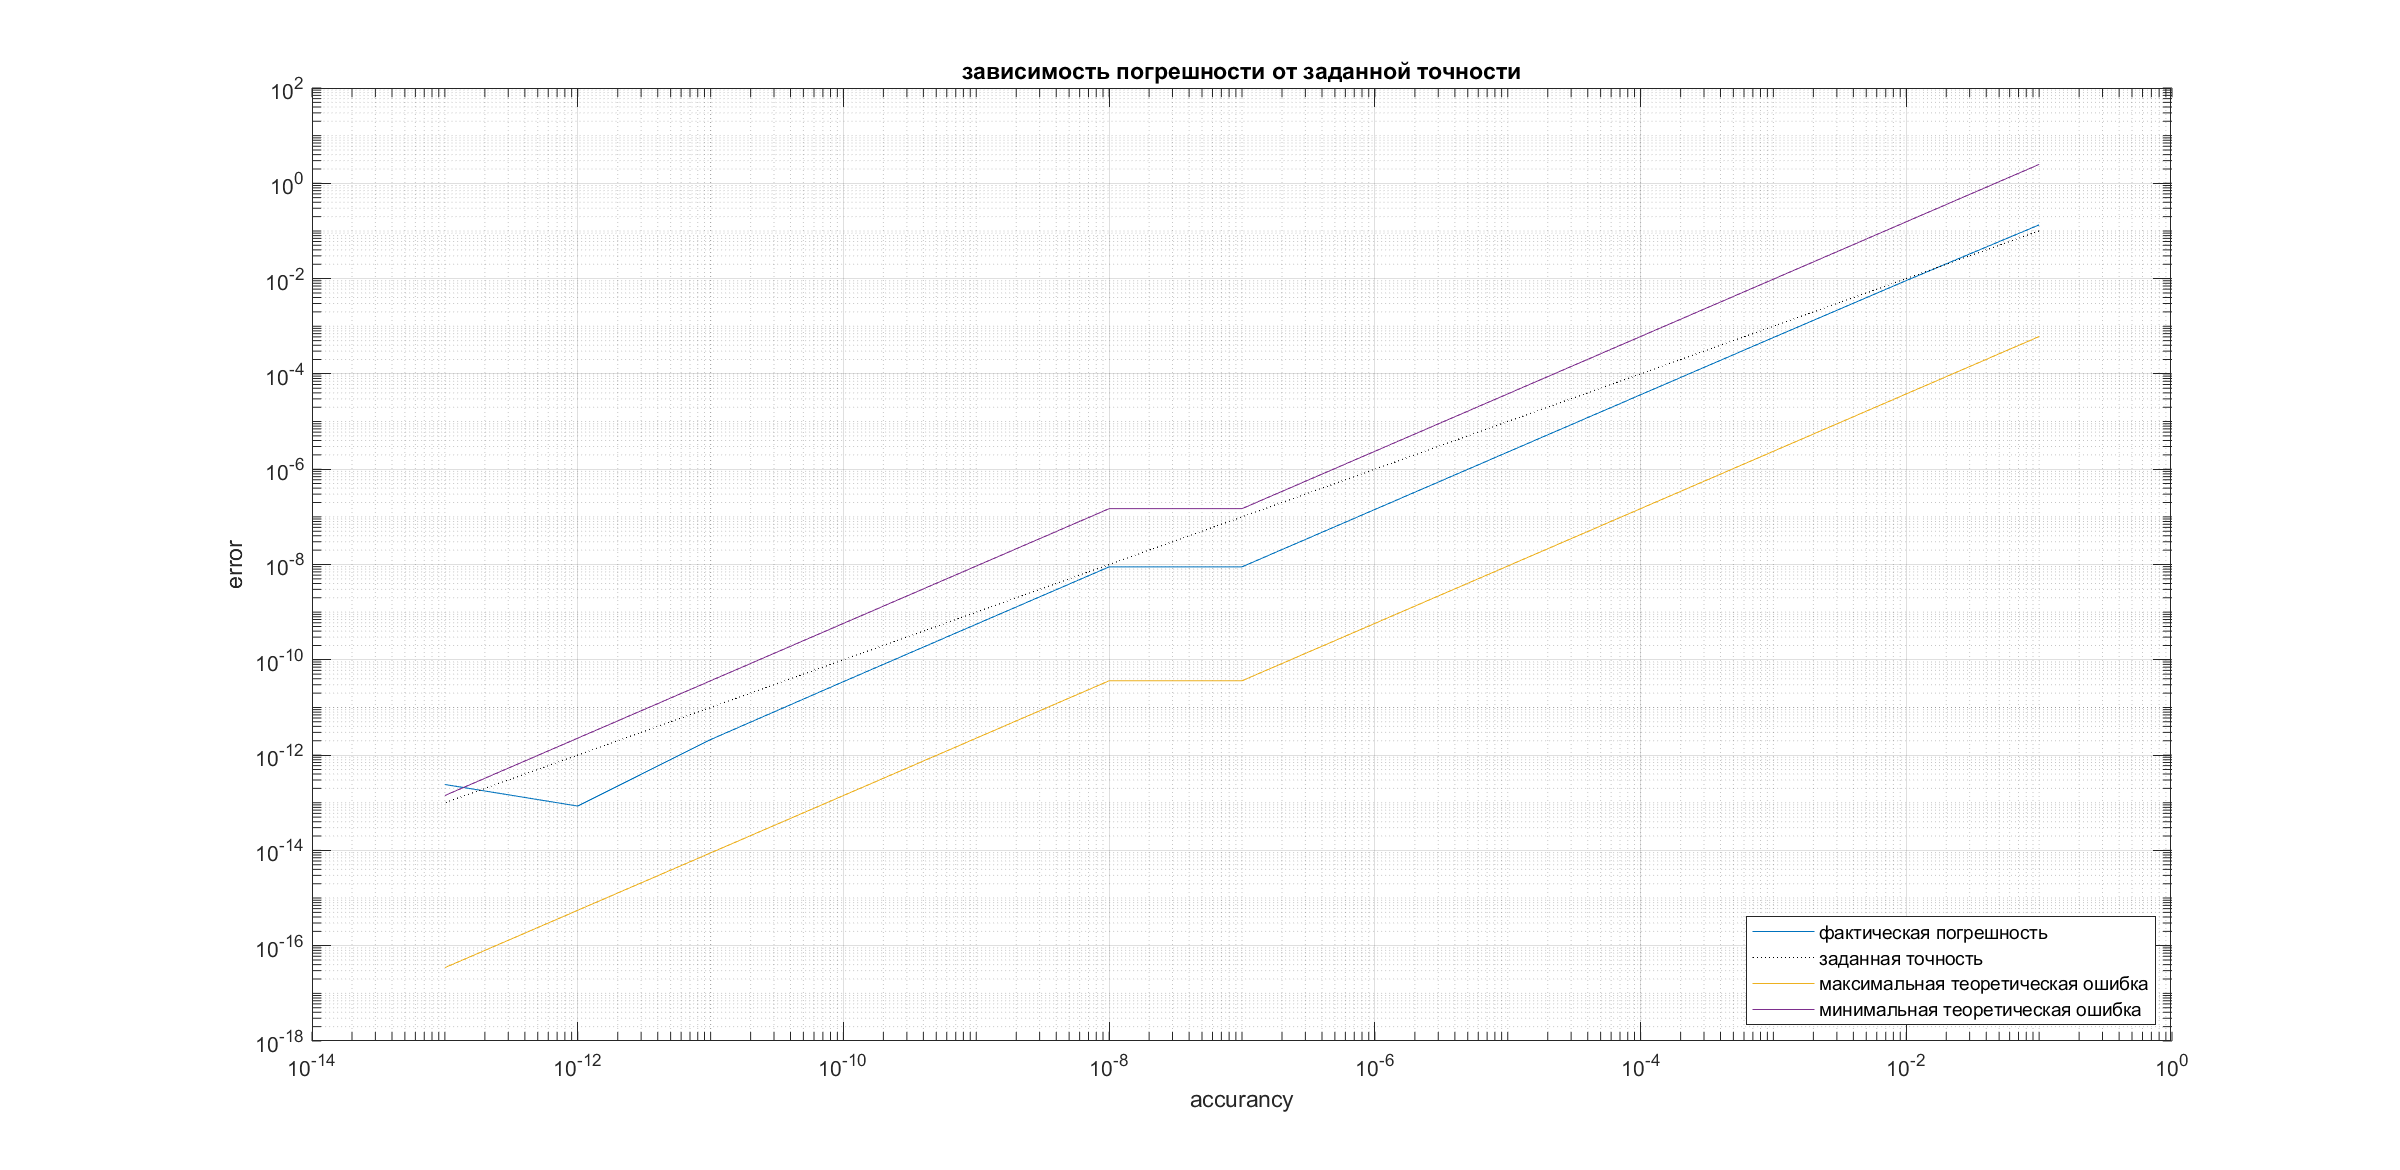
\includegraphics[scale = 0.4]{Погрешность} \end{center}
	Из графика видно, что все заданные точности достигаются, за исключением последней точки, что связано с ограниченной точностью типа данных double в языке C++.\\
	$\triangleright$ \underline{Количество разбиений:}\\
	\begin{center} 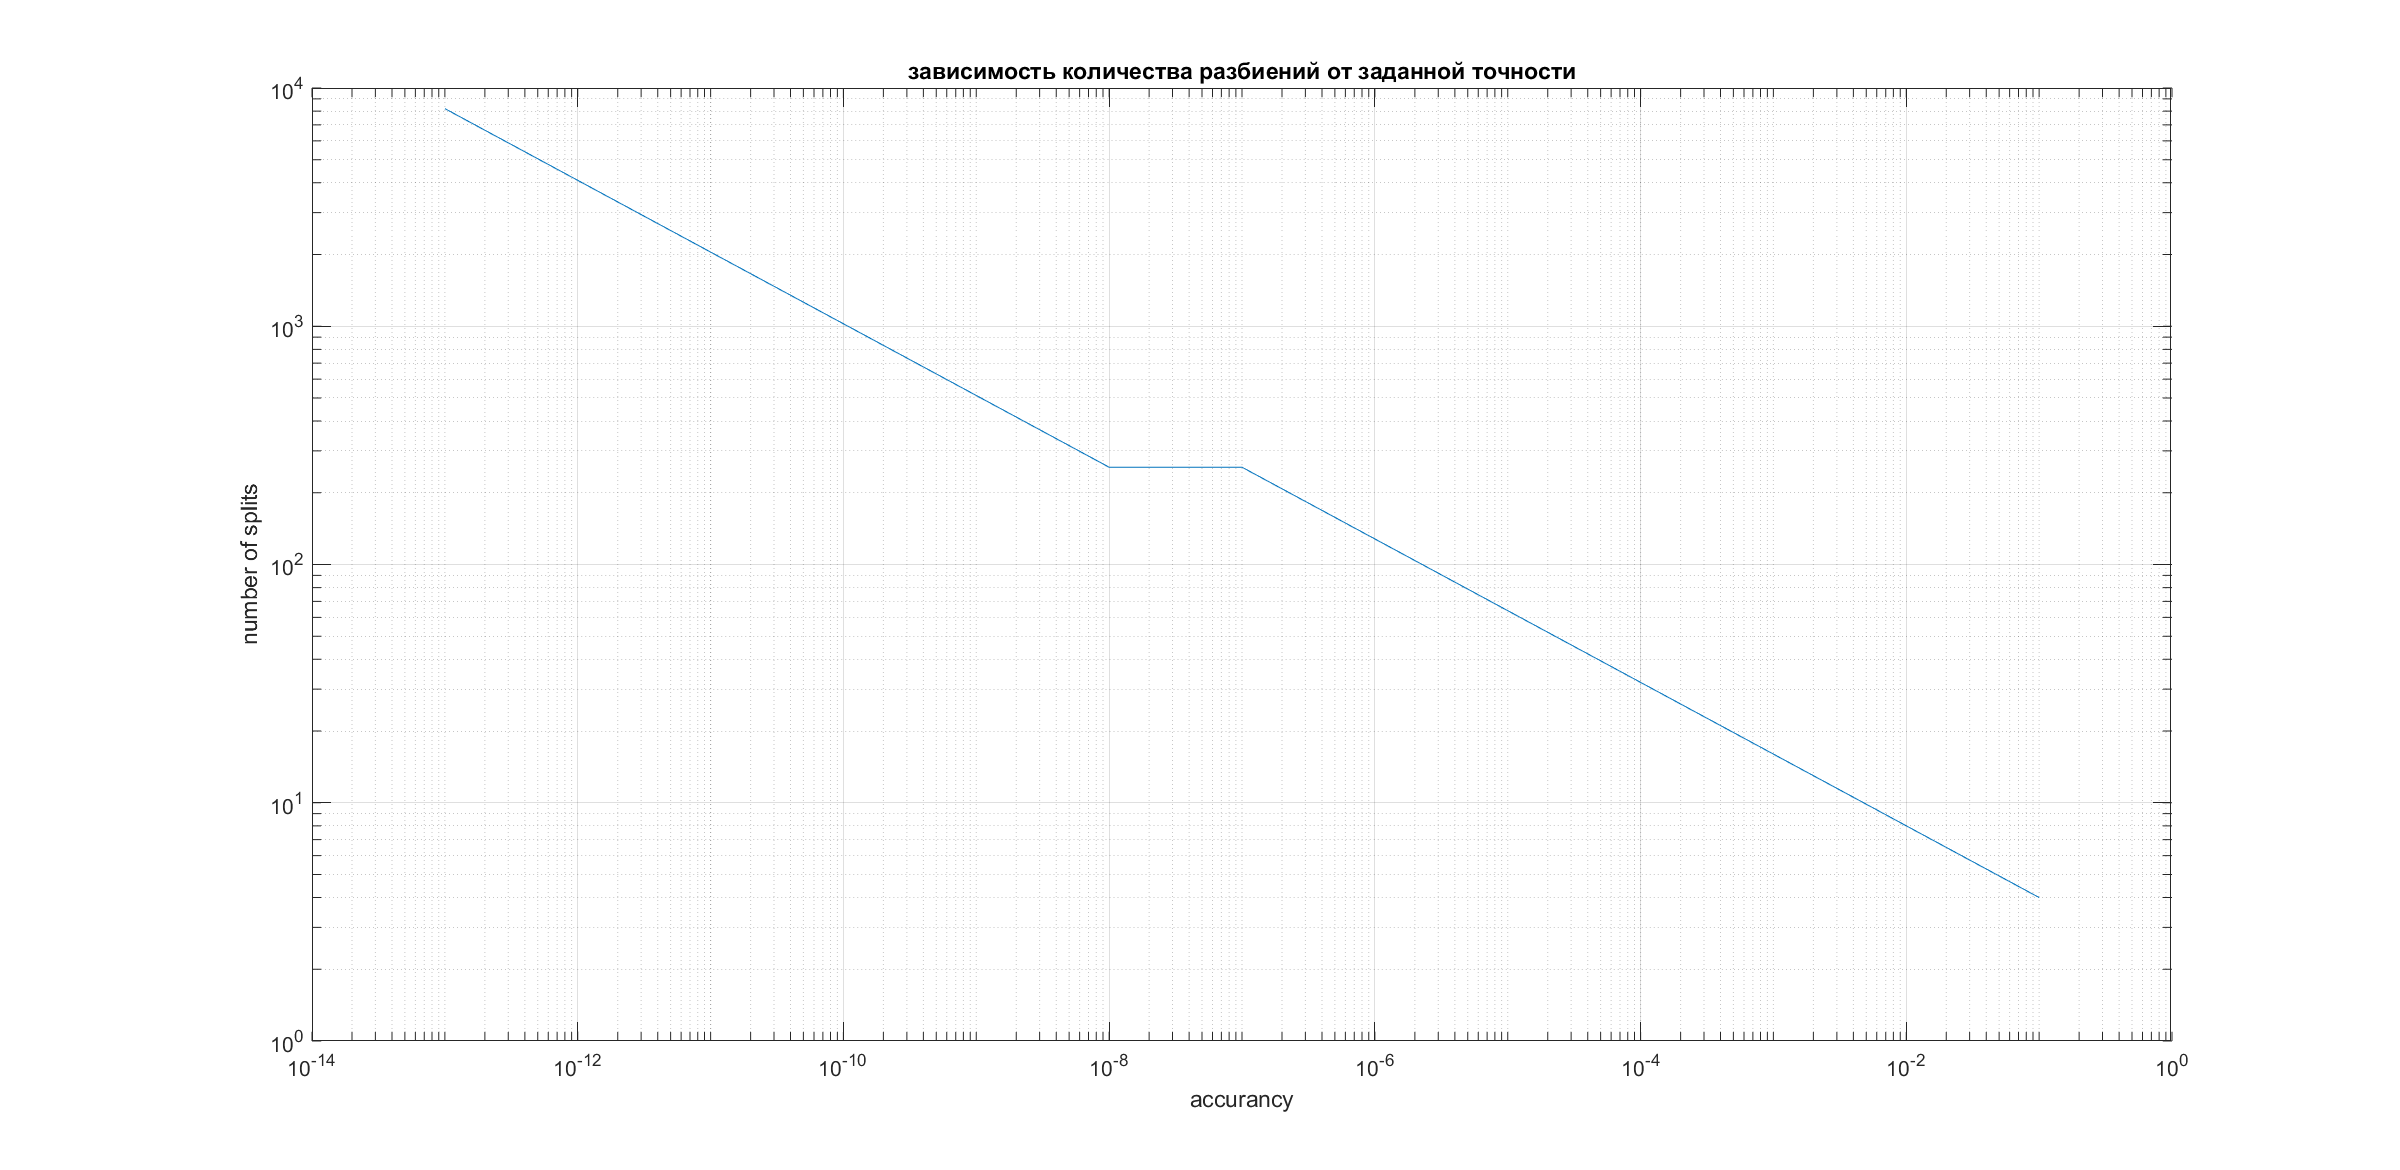
\includegraphics[scale = 0.4]{Разбиения} \end{center}
	По графику видно, что зависимость линейная и количество разбиений почти каждый раз растет в 2 раза.
	\begin{center} \textbf{Общие выводы}\end{center}
	В данной лабораторной работе мы научились численно вычислять опредленный интеграл на заданном промежутке с помощью формулы Чебышева для 3х точек. Реализация метода очень простая, что видно из модульной структуры. Метод довольно эффективный, но он проигрывает формулам Гаусса, где алгебраический порядок точности больше в 2 раза, хотя он реализуется труднее. 
\end{document}